\vspace{-2ex}
\section{Approach}
\label{sec:approach}
\vspace{-2ex}
\CodeIn{eXpress} takes as input the assembly code of two versions $v1$ (original) and $v2$ (new) of the program under test. In addition, \CodeIn{eXpress} takes as input, the name and signature of a parameterized unit test (PUT); such a PUT serves as a test driver for path exploration. 
When an existing test suite is available for the original version, \CodeIn{eXpress} conducts incremental exploration that exploits the test suite for generating tests for the new version. We next discuss in detail the \CodeIn{eXpress} approach. 


%The Difference Finder component finds the set of differences between each of the corresponding method pairs in the two versions of the program. The Graph Builder component builds an inter-procedural graph $G$ with the input PUT as the starting method. The Graph Traverser component traverses the graph to find all the branches $B_{E+I}$ that need not be explored for executing the changed regions and infect the program state and the branches $B_P$ that cannot help in propagating a state infection to an observable output. 
%The Instrumenter
%component instruments both versions of the program under test so
%that program states can be compared (to determine state infection).
%The Dynamic Test Generator generates tests for the input PUT, pruning branches $B_{E+I}$ from exploration before a test is generated that infects the program state. In addition, Dynamic Test Generator prunes branches $B_{P}$ after the program state
%is infected until a behavioral difference is found.

%\Comment{
%\begin{figure}[t]
%    \centering
%        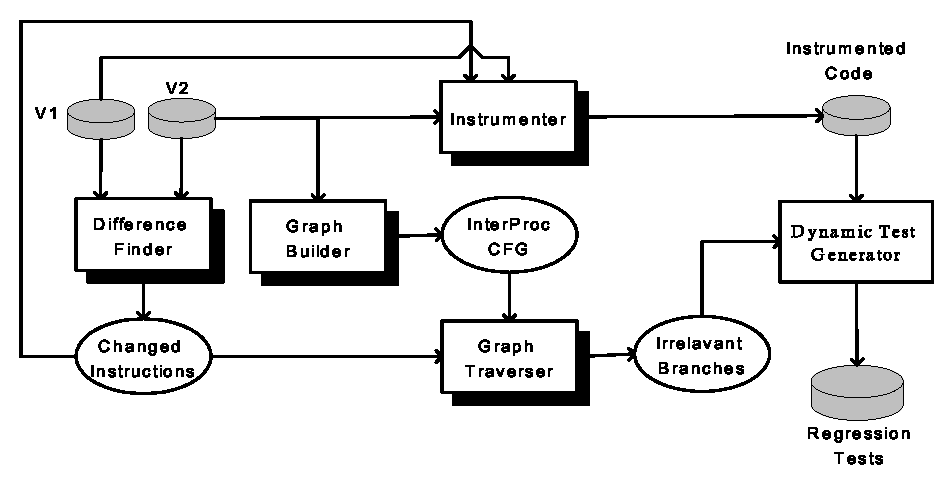
\includegraphics[width=8cm, keepaspectratio]{Figures/appr}
%        \vspace{-0.35 in}
%    \caption{Overview of \CodeIn{eXpress}}
%    \label{fig:approach}
%    \vspace{-0.15 in}
%\end{figure}
%}
\vspace{-2ex}
\subsection{Finding Differences Between Versions}
\vspace{-1.5ex}
\CodeIn{eXpress} analyzes the two versions $v1$ and $v2$ to find pairs $<$$M_{i1}, M_{i2}$$>$ of corresponding methods in $v1$ and $v2$, where $M_{i1}$ is a method in $v1$ and $M_{i2}$ is a method in $v2$. A method $M$ is defined as a triple $<$$FQN, Sig, I$$>$, where $FQN$ is the fully qualified name\footnote{\scriptsize{The fully qualified name of a method $m$ is a combination of the method's name, the name of the class $c$ declaring $m$, and the name of the namespace containing $c$.}} of the method, $Sig$ is the signature\footnote{\scriptsize{Signature of a method $m$ is the combination of parameter types of $m$ and the return type of $m$.}} of the method, and $I$ is the list of assembly instructions in the method body. Two methods $<$$M_{i1}, M_{i2}$$>$ form a  corresponding pair if the two methods $M_{i1}$ and $M_{i2}$ have the same $FQN$ and $Sig$. Currently our approach considers as different methods the methods that have undergone Rename Method or Change Method Signature refactoring. A refactoring detection tool~\cite{Dig'06:ECOOP} can be used to find such corresponding methods. For each pair $<$$M_{i1}, M_{i2}$$>$ of corresponding methods, the Difference Finder finds a set of  differences $\Delta_i$ between the list of instructions $I_{M_{i1}}$ and $I_{M_{i2}}$ in the body of Methods $M_{i1}$ and $M_{i2}$, respectively. $\Delta_i$ is a set of instructions such that each instruction $\iota$ in $\Delta_i$ is an instruction in $I_{M_{i2}}$ (or in $I_{M_{i1}}$ for a deleted instruction), and $\iota$ is added, modified, or deleted from list $I_{M_{i1}}$ to form $I_{M_{i2}}$. 
We denote the set of all added, modified, or deleted instructions as $\Delta$. 
%\subsection{Graph Builder}
%   
%The Graph Builder component makes an inter-procedural control flow graph (CFG) of the program version $v_2$. The Graph Builder component starts the construction of the inter-procedural CFG from the Parametrized Unit Test (PUT) $\tau$ provided as input. The inter-procedural CFG is used by the Graph Traverser component to find branches (in the graph) via which the execution cannot reach any vertex containing a changed instruction in the graph.
%\algsetup{indent=2em}
%\newcommand{\factorial}{\ensuremath{\mbox{\sc Factorial}}}
%\vspace{- 0.25 in}
%\begin{algorithm}[h!]
%\begin{tiny}
%\caption{$InterProceduralCFG(\tau)$}\label{alg:factorial}
%\begin{algorithmic}[1]
%\REQUIRE A test method $\tau$.
%\ENSURE The inter-procedural Control Flow Graph (CFG) of the program under test.
%
%\medskip
%
%\STATE $Graph$ $g \leftarrow GenerateIntraProceduralCFG$($\tau$)
%\FORALL {Vertex $v \in g.Vertices$}
%\IF{v.Instruction = MethodInvocation}
% \STATE $c \leftarrow getMethod(v.Instruction)$
% \IF {$c \in MethodCallStack$}
% \STATE $goto$ Line 2 //To avoid loops
% \ENDIF
% 
% 
% \IF{$c \in ReachableToChangedRegion$}
%  \STATE $g \leftarrow GraphUnion(ChangedMethod, g, v)$ 
%  \STATE $goto$ Line 2
% \ENDIF 
% 
% \IF{$c \in Visited$}
%  \STATE $goto$ Line 2
% \ENDIF 
% 
% \IF{$c \in ChangedMethods$}
%	 \STATE $ChangedMethod \leftarrow c $
%	 \FORALL {Method $m \in MethodCallStack$}
%		 \STATE $ReachableToChangedRegion.Add(m)$	
% 	 \ENDFOR
% \ENDIF
% 
% 
% 		
% \STATE $MethodCallStack.Add(c)$
% \STATE $cg \leftarrow InterProceduralCFG(c)$ 
% \STATE $MethodCallStack.Remove(c)$
% \STATE $Visited.Add(c)$
% 
% \STATE $g \leftarrow GraphUnion(cg, g, v)$
% \ENDIF
%\ENDFOR
%\RETURN $g$
%\caption{Pseudocode of Construction of Inter-Procedural Control Flow Graph}
%\label{alg:ICFG}
%\end{algorithmic}
%\end{tiny}
%\end{algorithm}
%Since a moderate-size program can contain millions of method calls (including those in its dependent libraries), often the construction of inter-procedural graph is not scalable to real-world programs. Hence, we build a minimal inter-procedural CFG for which our purpose of finding branches that cannot reach some changed region in the program can be served. The pseudo code for building the inter-procedural CFG is shown in Algorithm~\ref{alg:factorial}. Initially, the algorithm \CodeIn{InterProceduralCFG} is invoked with the argument as the PUT \CodeIn{$\tau$}. The algorithm first constructs an intra-procedural CFG $g$ for method $\tau$. 
%For each method invocation vertex\footnote{\scriptsize{A method invocation vertex is a vertex representing a call instruction.}} (invoking Method $c$) in $g$, the algorithm \CodeIn{InterProceduralCFG} is invoked recursively with the invoked method $c$ as the argument (Line 22 of Algorithm~\ref{alg:factorial}), after adding $c$ to the call stack (Line 21). After the control returns from the recursive call, the method $c$ is removed from the call stack (Line 23) and added to the set of visited methods (Line 24). The inter-procedural graph \CodeIn{cg} (with $c$ as an entry method) resulting from the recursive call at Line 22 is merged with the graph $g$ (Line 25).
%\Comment{
%To avoid loops in method invocations, the method \CodeIn{InterProceduralCFG} is not invoked recursively with $c$ as argument if $c$ is already in the call stack (Lines 5-6). In addition, thee method \CodeIn{InterProceduralCFG} is not invoked recursively with $c$ as argument if $c$ is already visited (Lines 23). 
%If a changed method\footnote{\scriptsize{A changed method $M_i$ is a method for which the difference set $\Delta_i \neq \phi $.}} is encountered, the methods in the call stack are added to the set \CodeIn{ReachableToChangedRegion} (Lines 17-19). Finally, if a method $c$ in \CodeIn{ReachableToChangedRegion} is encountered, the method \CodeIn{InterProceduralCFG} is not invoked recursively with $c$ as argument, while merging CFG of some changed method with $g$. Since our aim of building the intra-procedural graph is to find branches in the graph that are not reachable to any changed instruction, the previous step helps in achieving the aim while reducing the cost of building the inter-procedural CFG. In addition, the size of the inter-procedural graph is also reduced which results in reduction in the cost of finding branches not reachable to the changed instructions.
%}
%The algorithm \CodeIn{InterProceduralCFG} is not invoked recursively with $c$ as argument in the following situations:
%\begin{itemize}
%\\ \textbf{$c$ is in call stack.} If $c$ is already in the call stack, \CodeIn{InterProcedural CFG} is not recursively invoked with $c$ as argument (Lines 5-6). This technique ensures that our approach is not stuck in a loop in method invocations. For example, if method A invokes method B, and method B invokes A, then the construction of the inter-procedural graph stops after A is encountered the second time.
%\\ \textbf{ $c$ is already visited.} If $c$ is already visited, \CodeIn{InterProcedural CFG} is not recursively invoked with $c$ as argument (Line 23). This technique ensures that we do not build the same subgraph again.
%\\ \textbf{ $c$ is in \CodeIn{ReachableToChangedRegion}.} The set \CodeIn{ReachableToChanged Region} is populated whenever a changed method\footnote{\scriptsize{A changed method $M_i$ is a method for which the set $\Delta_i \neq \phi $.}} is encountered. In particular, if a changed method is encountered, the methods currently in the call stack are added to the set  \CodeIn{ReachableToChanged Region} (Lines 17-19). If $c$ is in \CodeIn{ReachableToChangedRegion}, \CodeIn{InterProceduralCFG} is not recursively invoked with $c$ as argument, while merging CFG of some changed method with $g$ (Line 8-11).
%Note that if a method \CodeIn{m} can reach a changed method \CodeIn{cm}, all the branches in this method \CodeIn{m} may not be able to reach \CodeIn{cm} (for example, due to $return$ statements). Branches that cannot reach any changed region (irrelevant branches) are found by the Graph Traverser component.  
%
%\end{itemize}
%If a branching node $b$ can reach a changed region in Inter-Procedural CFG $g1$ built without using the preceding optimization, the branching node $b$ can reach a changed region (maybe a different one) in graph $g2$ built using the preceding optimizations. 
%Since our aim of building the intra-procedural CFG is to find irrelevant branches, those in the graph via which the execution cannot reach any changed region, the preceding three optimizations help achieve the aim while reducing the cost of building the inter-procedural CFG. In addition, the size of the inter-procedural CFG is reduced resulting in reduction in the cost of finding irrelevant branches.

\vspace{-1ex}
\subsection{Finding Irrelavant Branches.}
\vspace{-2ex}
\CodeIn{eXpress} efficiently constructs the inter-procedural CFG $g<$$V,E$$>$ of 
the new version of the program under test such that each vertex $v \in V$ 
corresponds to an instruction $\iota \in M$ (denoted as $v \leftrightarrow \iota$), where $M$ is some method in $v_2$.  
\CodeIn{eXpress} traverses the graph $g$ to find a set of branches $B_{E+I}$ via which the execution cannot reach any of the branches in $V$ and a set of branches $B_{P}$ via which a state infection cannot propagate to any observable output. A branch $b$ in CFG $g$ is an edge $e = <$$v_i, v_j$$>: e \in E$ , $v_i \in V$ with an outgoing degree of more that one. The vertex $v_i$ is referred to as a branching node. 
We next describe the sets $B_{E+I}$ and $B_P$.

Let $V=\{v_1,v_2,..,v_l\}$ be the set of all vertices in CFG $g$$<V, E$$>$ such that $ v_i \in V$ and $v_i.degree >1$ . Let $E_i = \{e_{i1}, e_{i2},...,e_{im}\}$ be the set of outgoing edges (branches) from $v_i$. Let $C$ be the set of vertices in the CFG $g$ 
such that $\forall v \in C, \exists \iota \in \Delta : v \leftrightarrow \iota$.  $\rho(v_i, v_j, e_{ij})$ denotes a path between a source vertex $v_i$ to a destination vertex $v_j$ that takes the branch $e_{ij}$ (if $\rho(v_i, v_j, e_{ij}) =\phi$, there is no such path from $v_i$ to $v_j$), $\rho(v_i, v_j)$ denotes a path from a source vertex $v_i$ to a 
destination vertex $v_j$(if $\rho(v_i, v_j)=\phi$, there is no such path from $v_i$ to $v_j$).
\\ \textbf{Branches $B_{E+I}$. } 
$B_{E+I} \subseteq E$ is a set of branches such that $\forall e_{ij} = $$<v_i, v_j$$> \in B_{E+I} 
\wedge \forall c_k\in C: \rho(v_i, c_k, e_{ij}) = \phi$. 
Since $\rho(v_i, c_k, e_{ij}) = \phi$, after taking a branch $e_{ij} \in  B_{E+I}$, the
program execution cannot reach a changed region. Hence, the program state cannot be infected. 
\\ \textbf{Branches $B_P$. }
$B_{P} \subseteq E$ is a set of branches such that $\forall e_{ij} = $$<v_i, v_j$$> \in B_{P} 
\wedge \forall c_k\in C: \rho(v_i, c_k, e_{ij}) = \phi \wedge \rho(c_k, v_i) = \phi$. 
Since $\rho(c_k, v_i) = \phi$, a state infection after a changed vertex $c_k$ cannot reach $v_i$. 
Hence, the state infection cannot propagate through $e_{ij}$.



%The pseudo code for finding the set of branches $B_{E+I}$ and $B_P$ is shown in Algorithm~\ref{alg:irrelavantBranches}.
%
%\algsetup{indent=2em}
%\newcommand{\UnrechableBranches}{\ensuremath{\mbox{\sc FindUnreachableBranches}}}
%\begin{algorithm}[h!]
%\begin{tiny}
%\caption{$FindUnreachableBranches(g, V)$}\label{alg:irrelavantBranches}
%\begin{algorithmic}[1]
%\REQUIRE A Graph $g$ and a set $V$ of vertices in Graph $g$.
%\ENSURE A set of branches $B_{E+I}$ in Graph $g$ that do not have a path to any vertex $v \in V$ and a set of branches 
%$B_P$ that do not have a path to and from any vertex $v \in V$.
%
%\medskip
%
%\STATE $Reachable \leftarrow Reachable \cup V$
%\FORALL {Vertex $v \in g.Vertices$ such that $v.degree > 1 $}
%  
%  \IF {$Reachable.Contains(v)$}
%  	\STATE goto Line 2
%  \ENDIF
%  
%	\STATE $\rho \leftarrow FindPathUsingDFS(v, V, Reachable)$
%	\STATE $\rho' \leftarrow FindPathUsingDFS(V, v, Reachable')$
%	
%	\IF {$\rho$ is empty}
%	  \FORALL {Vertex $n \in v.OutVertices$} 
%			\STATE $B_{E+I} \leftarrow B_{E+I} \cup <v,n>$
%			\IF {$\rho'$ is empty}
%				\STATE $B_{P} \leftarrow B_{P} \cup <v, n>$
%			\ENDIF	
%		\ENDFOR
%   	\STATE goto Line 2
%	\ENDIF
%		
%	\FORALL {Vertex $pv \in \rho$ such that $v.degree > 1 $}
%		\STATE $Reachable \leftarrow Reachable \cup pv$
%	\ENDFOR
%	\FORALL {Vertex $pv' \in \rho'$ such that $v.degree > 1 $}
%		\STATE $Reachable' \leftarrow Reachable' \cup pv'$	
%	\ENDFOR
%	
%	\WHILE {$v.OutVertices \neq \phi$} 
%	    \STATE $R \leftarrow R \cup <v, v_j>: v_j \in \rho$
%			\STATE $g \leftarrow g.RemoveEdge(v, v_j)$
%			\STATE $\rho \leftarrow FindPathUsingDFS(v, V, Reachable)$
%			\STATE $\rho' \leftarrow FindPathUsingDFS(V, v)$
%			\IF{$\rho$ is empty}
%					\FORALL {Vertex $o \in v.OutVertices$}
%						\STATE $B_{E+I} \leftarrow B_{E+I} \cup <v, o>$
%						\IF {$\rho'$ is empty}
%							\STATE $B_{P} \leftarrow B_{P} \cup <v, o>$
%						\ENDIF	
%					\ENDFOR
%					\STATE $g \leftarrow g.AddEdges(R$)
%					\STATE goto Line 2
%			\ENDIF	
%	\ENDWHILE
%	\STATE $g \leftarrow g.AddEdges(R)$	
%\ENDFOR
%\RETURN $B$
%\label{alg:ICFG}
%\end{algorithmic}
%\end{tiny}
%\end{algorithm}


%For each Vertex $v$ in $g$ where $degree(v) > 1$, the Graph Traverser performs a depth-first search (DFS) from Vertex $v$ (Line 6) to find a path between $v$ and some vertex $c \in V$.
%\Comment{ (the pseudo code of DFS is shown in Algorithm~\ref{alg:DFS}).
%\algsetup{indent=2em}
%\newcommand{\DFS}{\ensuremath{\mbox{\sc DFS}}}
%\begin{algorithm}[h!]
%\begin{tiny}
%\caption{$FindPathUsingDFS(g, v, R)$}\label{alg:DFS}
%\begin{algorithmic}[1]
%\REQUIRE A Graph $g$, a vertex $v$ in the graph $g$, a set of vertices $R$.
%\ENSURE A path $\rho$ in Graph $g$ from Vertex $v$ to Vertex $c \in V$.
%
%\medskip
%
%\STATE $v.Visited \leftarrow true$;
%\STATE $\rho$.Append(v)
%\IF {$v \in R$}
%	\RETURN $\rho$
%\ENDIF	
%\FORALL {Vertex $n$ in v.OutVertices}
%	\IF{$n.Visited \neq true$}
%		\STATE goto Line 6 
%	\ENDIF
%	\STATE $\rho$.Append(n);
%	\IF {$n \in R$}
%		\RETURN $\rho$
%	\ENDIF
%	\STATE $\varrho \leftarrow FindPathUsingDFS(g, n, R)$
%	\IF {$\varrho$ is not empty}
%	  \RETURN $\varrho$
%	\ENDIF
%	\STATE $\rho.Remove(n)$
%
%\ENDFOR
%\STATE $\rho$.Remove(v)
%\RETURN $\phi$
%\label{alg:ICFG}
%\end{algorithmic}
%\end{tiny}
%\end{algorithm}
%}If no path is found, all branches $b_i = <v, v_i>$ are added to the set $B_{E+I}$ (Lines 8-10) since none of these branches have a path to any of the vertices in $V$. In addition if there is no path from any vertex in $V$ to $v$, branch 
% all branches $b_i = <v, v_i>$ are added to $B_{P}$. 
%
%If a path $\rho$ is found by the DFS, there may still be a branch $b_i = <v, v_i>$ that cannot reach any vertex $c \in V$. To find such a branch, we remove each edge $e_j=<v, v_j>: e_j \in \rho$ one at a time from the graph and perform DFS again starting from $v$ (Lines 23-38). We repeat the preceding steps until we either find no path $\rho$ or all the edges from $v$ are removed from the graph. If no path is found, the remaining edges (branches) from v are added to the set $B_{E+I}$ (Lines 29-30) and to the set $B_{P}$ is there is no path from all vertices $c \in V$ to $v$ (Lines 31-32).

%The Graph Traversal component uses Depth First Search on the Graph $g$ to efficiently find the sets $B_{E+I}$ and $B_P$.
\vspace{-2ex}
\subsection{Code Instrumentation}
\vspace{-2ex}
For each changed method pair $<$$M_{i1}, M_{i2}$$>$ for which $\Delta_i \neq \phi$, \CodeIn{eXpress} finds changed regions $\delta_{i1}$ and $\delta_{i2}$ (for original and new program version, respectively) 
containing all the changed instructions in the program. 
A changed region $\delta_i$ is a minimal list of continuous instructions 
such that all the changed instructions in the method $M_i$ are in the 
region $\delta_i$. Hence, there can be a maximum of one changed region in one method.
Inputs $I = \{i_1, i_2...,i_n\}$ of a changed region $\delta$ are variables (or fields) that are used 
in the changed region $\delta$ but are declared outside the changed region, 
while outputs $O = \{o_1, o_2...,o_m\}$ are variables (or fields) 
that are defined in $\delta$ and used outside the changed region.
As an example, for the changed region in the new version of \CodeIn{TestMe} in Figure~\ref{fig:example}, $I = \{c.Length, n, state\}$ and $O = \{state\}$.
Let $I_1$ and $O_1$ be the inputs and outputs of $\delta1$, while $I_2$ and $O_2$ be 
the inputs and outputs of $\delta2$, respectively.

\CodeIn{eXpress} extracts the instructions in $\delta_{i1}$ and $\delta_{i2}$ as methods $M_{\delta_{i1}}$ and 
$M_{\delta_{i2}}$ (shown in Figure~\ref{fig:instrumented}), respectively, both having arguments of type and name as $I_1 \bigcup I_2$ and returning outputs 
$O_1 \bigcup O_2$.
We refer to the arguments of $M_{\delta_{i1}}$ as $A_{1} = {i_{11}, i_{21},...,i_{n1}}$ and the arguments of 
$M_{\delta_{i2}}$ as $A_{2} = {i_{12}, i_{22},...i_{n2}}$, such that the types of $i_{l1}$ and $i_{l2}$
are same as the type of $i_l \in I_1 \bigcup I_2$.
We refer to the variables corresponding to $o_i \in O_1 \bigcup O_2$ in $M_{\delta_{i1}}$ as $o_{i1}$ and in 
$M_{\delta_{i2}}$ as $o_{i2}$.
\CodeIn{eXpress} synthesizes a class $C_o$ (show in Figure~\ref{fig:instrumented}), such that 
for all $o_i \in O_1 \bigcup O_2$, there is a corresponding public field in $C_o$ with 
types and names same as $o_i$.
The methods $M_{\delta_{i1}}$ and $M_{\delta_{i2}}$ return an object $c_o$ of type $C_o$.
The class enables the two methods $M_{\delta_{i1}}$ and $M_{\delta_{i2}}$
to return multiple outputs $O_1 \bigcup O_2$ as fields of $C_o$.
As shown in Figure~\ref{fig:instrumented}, the method $M_{\delta_{i1}}$ (and $M_{\delta_{i2}}$)
first contains the instructions in $\delta_{i1}$ and later copies all the outputs 
$o_{i1}$ in $M_{\delta_{i1}}$ ($o_{i2}$ in $M_{\delta_{i2}}$) to the respective fields 
of $c_o$ and returns the object $c_o$.


Figure~\ref{fig:instrumented} shows the instrumented part of the method $M_{i2}$. 
The methods $M_{\delta_{i1}}$ and $M_{\delta_{i2}}$ are invoked (Lines 5 and 6 of the Method $M_{i2}$ in Figure~\ref{fig:instrumented}) from the method $M_{i2}$ instead of the changed region.
For the method $M_{\delta_{i2}}$, $i_1,....i_n$ are passed as arguments, while for the method $M_{\delta_{i1}}$
copied values $i_{1c},....i_{nc}$ of $i_1,....i_n$ are passed as arguments (Lines 1 to 4). These copies are deep copies for non primitive type variables.
The outputs of $M_{\delta_{i1}}$ and $M_{\delta_{i2}}$ are stored in objects $c_{o}Old$ and $c_{o}New$, respectively.
An \CodeIn{if} statement is inserted (Line 7) such that its \CodeIn{true} branch is executed when the outputs 
$c_{o}Old$ and $c_{o}New$ are different.    
To compare the two outputs, \CodeIn{eXpress} changes modifiers 
of all fields transitively reachable from objects of the
two given classes to \CodeIn{public} and compares these fields directly to detect difference in the outputs.
Finally, the fields of $c_{o}New$ are assigned to the corresponding output variables (Lines 8 to 10).



\begin{figure}[t]
%  \begin{\begin{center}
\hspace{0.5cm}
	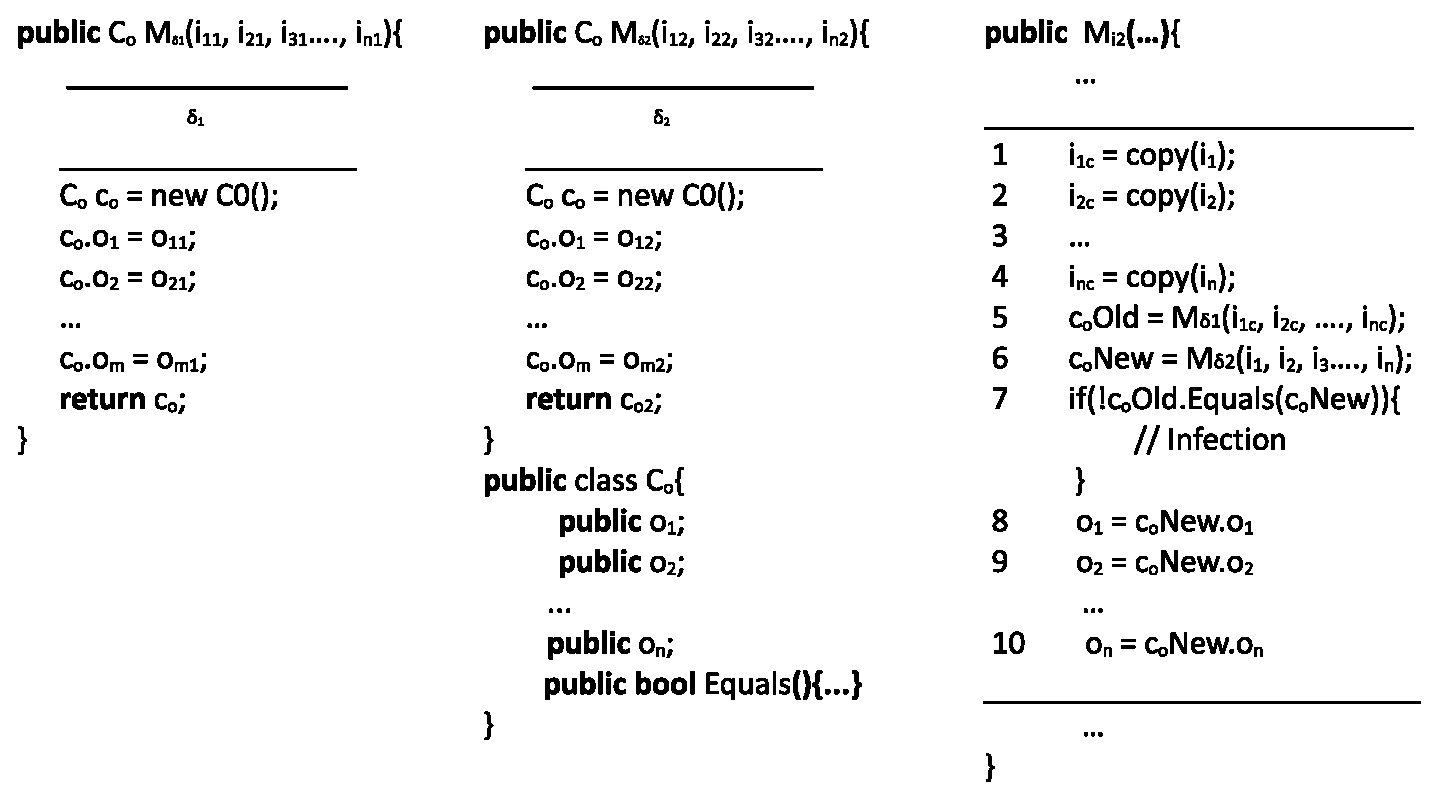
\includegraphics[width=11cm, keepaspectratio]{Figures/instrumentation}
  
\vspace{-0.15 in}
\caption{Instrumented Code synthesized by \CodeIn{eXpess}}
\label{fig:instrumented}
\vspace{-0.25 in}
%\end{center}
\end{figure}


%The Instrumenter component uses Sets $\Delta_i$ (differences between method $M_{i1}$ and $M_{i2}$) produced by the Difference Finder. For each changed method pair $<M_{i1}, M_{i2}>$ for which $\Delta_i \neq \phi$, the Instrumenter component finds a region $\delta_i$ containing all the changed instructions in the program. $\delta_i$ is a minimal list of continuous instructions such that all the changed instructions in the method $M_i$ are in the region $\delta_i$. Hence, there can be a maximum of one changed region in one method. At the end of each changed region $\delta_i$, the Instrumenter component inserts instructions to save the program state. In particular, the Instrumenter inserts the corresponding instructions for \CodeIn{PexStore} statements for each variable (and field) defined in the changed region.
%The \CodeIn{PexStore} statement for a variable $x$ results in an assertion statement \CodeIn{PexAssert.IsTrue( "uniqueName", x == currentX)} in the generated test, where \CodeIn{currentX} is the value of $x$ in the new version.
%The Dynamic Test Generator component generates tests for the new version $v2$.
%After the Dynamic Test Generator component generates a test that executes a changed region (note that in $v1$, we do not have a changed region), 
%the component executes the test on Version $v1$ 
%to compare program states after the execution of the changed region
%with the ones captured in the execution of Version $v2$. The instrumentation enables us to perform only one instance of DSE on the new version instead of performing two instances of DSE: one on the original and the other on the new program version. Performing two instances of DSE can be technically challenging since we have to perform the two DSE instances in a controlled manner such that both versions are executed  with the same input and the execution trace is monitored for both the versions by a common exploration strategy to decide which branching node to flip next in the two versions.
\vspace{-3ex}
\subsection{Test Generation}
\vspace{-2ex}
\CodeIn{eXpress} performs Dynamic Symbolic Execution (DSE)~\cite{dart,cute,exe} to 
generate regression tests for the two given versions of a program. DSE iteratively generates test inputs to cover various feasible paths in the program under test (the new version in our approach). In particular, DSE flips some branching node discovered in previous executions to generate a test input for covering a new path. 
%The branching node to be flipped is decided by a search strategy such as depth-first search.
%The exploration is quite expensive since there are an exponential 
%number of paths with respect to the number of branches in a program.
% However, the execution of many branches often cannot help in detecting behavioral differences. 
% In other words, covering these branches does not help in satisfying any of the condition E or I in the PIE model described in Section~\ref{sec:intro}. 
% Therefore, we do not flip such branching nodes in our new search strategy for generating test inputs that detect 
% behavioral differences between the two given versions of a program. Recall that, we refer to such branches as irrelevant branches. We next describe the two categories of paths that our approach avoids exploring. We then describe our incremental exploration technique when an existing test suite is available for the original version.
To make path exploration efficient in finding behavioral differences, 
\CodeIn{eXpress} avoids from exploring the following categories of paths:
 \Comment{
%\begin{itemize}
\\ \textbf{Rationale E: Paths not leading to any changed region.} Paths that cannot reach any changed region (denoted as $\delta$) need not be 
explored. For example, consider the \CodeIn{testMe} program in Figure~\ref{fig:example}.
 The changed statement is at Line 11 ($\delta$). While searching for a path 
 to cover $\delta$, we do not need explore paths containing the \CodeIn{true} branch of the condition at Line 8. 
\\ \textbf{Rationale I: Paths not causing any state infection.} Suppose that we cover $\delta$ at Line 11 
in Figure~\ref{fig:example} using inputs \CodeIn{x=90} and the array \CodeIn{y} of length 20 where each element of \CodeIn{y} has a value 15. The execution takes a path $P$ 
executing the loop 20 times, assigning the variable \CodeIn{x} to 110 and eventually 
covering $\delta$ at Line 11 . However, the program state after the execution of $\delta$ is not infected since 
after the first execution of $\delta$, the value of \CodeIn{x} is 3 in both versions. We need not explore the subpaths after the execution of a changed region that does not cause any state infection if these subpaths do not lead to any other changed region.
\Comment{
\item \textbf{Rationale P: Paths not propagating state infection to any observable output.} Suppose $\delta$ is executed, the program state is infected after the execution of $\delta$, but the infection does not propagate to an observable output. Let $\chi$ be the statement at which infection propagation stops. We need not explore the subpaths after the execution of $\chi$ if these subpaths do not lead to any other changed region.	 
}
%\end{itemize}
\subsubsection{Branching Nodes being Pruned}
In DSE, path exploration is realized by flipping branching nodes. We next describe two categories of branching nodes that we avoid flipping corresponding to the preceding two categories of paths that we intend to avoid exploring.
}
%\begin{itemize}
\\ \textbf{Category E+I.} \CodeIn{eXpress} does not explore these paths until a test 
is generated that infects the program state. Our approach avoids exploring all the branches in $B_{E+I}$. In other words, if a branching node $v_i$ is in the built dynamic execution tree\footnote{\scriptsize{A dynamic execution tree is the tree formed from the paths executed in the previous executions. Multiple instances $c_{i1}, c_{i2}, ..., c_{in}$ of a node $c_i$ in CFG can be present in a dynamic execution tree due to loops in a program.}}, such that the branch $e_{ij} \in B_{E+I}$ is not explored yet, our approach does not flip $v_i$ to make program execution take branch $e_{ij}$.
As an effect, our approach helps reduce the number of paths to be explored by avoiding the paths $P \in g : e_{ij} \in P$ until a test is generated that infects the program state.
\Comment{
\textbf{Category EI. }
Let $C \in g$ be the set of nodes in all the changed regions.
Let some $c_i \in C$ be executed, i.e., at least one instance $c_{ij}$ of $c_i$ is present in the dynamic execution tree $T$. Consider that the program state is not infected after the execution of the changed region containing $c_i$. Our approach prunes all the branching nodes $B \in T$, such that for all $b_i \in B: \rho(c_{ij}, b_i) \neq \phi , b_i \notin C $, where $\rho(c_i, b_i)$ is the path between the vertices $c_i$ and $b_i$ (if the path exists) in $T$. As an effect of pruning $B$, our approach does not explore the subpaths after a changed region's execution that does not cause any state infection.
}
\\ \textbf{Category P. }
\CodeIn{eXpress} does not explore these paths after a test is generated that infects the program state.
Our approach avoids exploring all the branches 
$e_{ij}\in B_p$. In other words, if a branching node $v_i$ is in the built dynamic execution tree such that one of its branch $e_{ij}$ is not explored yet, our approach does not flip $v_i$ to make program execution take branch $e_{ij}$.
As an effect, our approach helps reduce the number of paths to be explored by avoiding the paths $P \in g : e_{ij} \in P$.
These paths cannot help in propagating a state infection to an observable output.
%\end{itemize}

%\end{itemize}
\vspace{-2ex}
\subsection{Incremental Exploration}
\vspace{-2ex}
\label{sec:incremental}
A regression test suite achieving high code coverage may be available along with the original version of  a program. 
%This test suite may be manually written or generated by an automated test generation tool for the original version. 
However, the existing test suite might not be able to cover all the changed regions of the new version of the program. Our approach can reuses the existing test suite so that changed regions of the program can be executed efficiently due to which test generation is likely to find behavior differences earlier in path exploration. Our approach executes the existing test suite to build an execution
tree for the tests in the test suite. Our approach then starts the program
exploration using the dynamic execution tree instead of starting from an empty
tree. Our approach of seeding test inputs can help efficiently cover the changed regions of the program with two major reasons:
\\ \textbf{Discovery of hard-to-discover branching nodes.} By seeding the existing test suite for Pex to start exploration with, our approach executes the test suite to build an execution tree of the program. Some of the branching nodes in the built execution tree may take a large number of DSE runs (without seeding any tests) to get discovered. Flipping some of these discovered branching nodes nearer in CFG to the changed parts of the
program has more likelihood of covering the changed regions of the program~\cite{burnim}. Although, our approach currently does not specifically prioritize flipping of branching nodes near the changed regions, our approach can help these branching nodes to get discovered (by executing the existing test suite), which might take large number of DSE runs as shown in the example in Section~\ref{sec:example}.
\\ \textbf{Priority of DSE to cover not-covered regions of the program.} DSE techniques employ branch prioritization so that a high coverage can be achieved faster due to which DSE techniques choose a branch from the execution tree (built thus far) that have a high likelihood of covering changed regions (that are not covered by existing test suite for the original version). By seeding the existing test suite to program exploration, the DSE techniques do not waste time on covering the regions of the program already covered by the existing test suite. Instead, the DSE techniques give high priority to branching nodes that can cover not-covered regions of the program, which include the changed parts. Hence, the changed parts are likely to be covered earlier in path exploration.
 
 
\Comment{
Pex then focuses on flipping the unexplored branches to effectively cover the changed parts of the program.
Even seeding a single test that covers portions of the program neared in CFG to the changed parts  can help the program exploration in effectively covering the changed parts of the program because various branches are discovered in the execution tree that are, which otherwise might take a number of runs in .
Hence choosing the number of tests in the test suite to seed is an optimization problem. In section, ??? we conduct experiments by increasing the number of seeds. by seeding (1)one closest pest to the changes (2) seeding tests that achieve a high block coverage (3) seeding tests that achieve a higher path coverage, to assess whether seeding more tests helps the path exploration.
We found out that tests achieving a high block coverage performs the best.
}


 
 